\subsection{(W) Map obstacles}\label{s:mapObstacles}
    \noindent Define certainty of obstacles from map (\emph{Data fusion}), (reuse some content from Linkoping work)
    \begin{figure}[H]
        \begin{subfigure}{0.32\textwidth}
            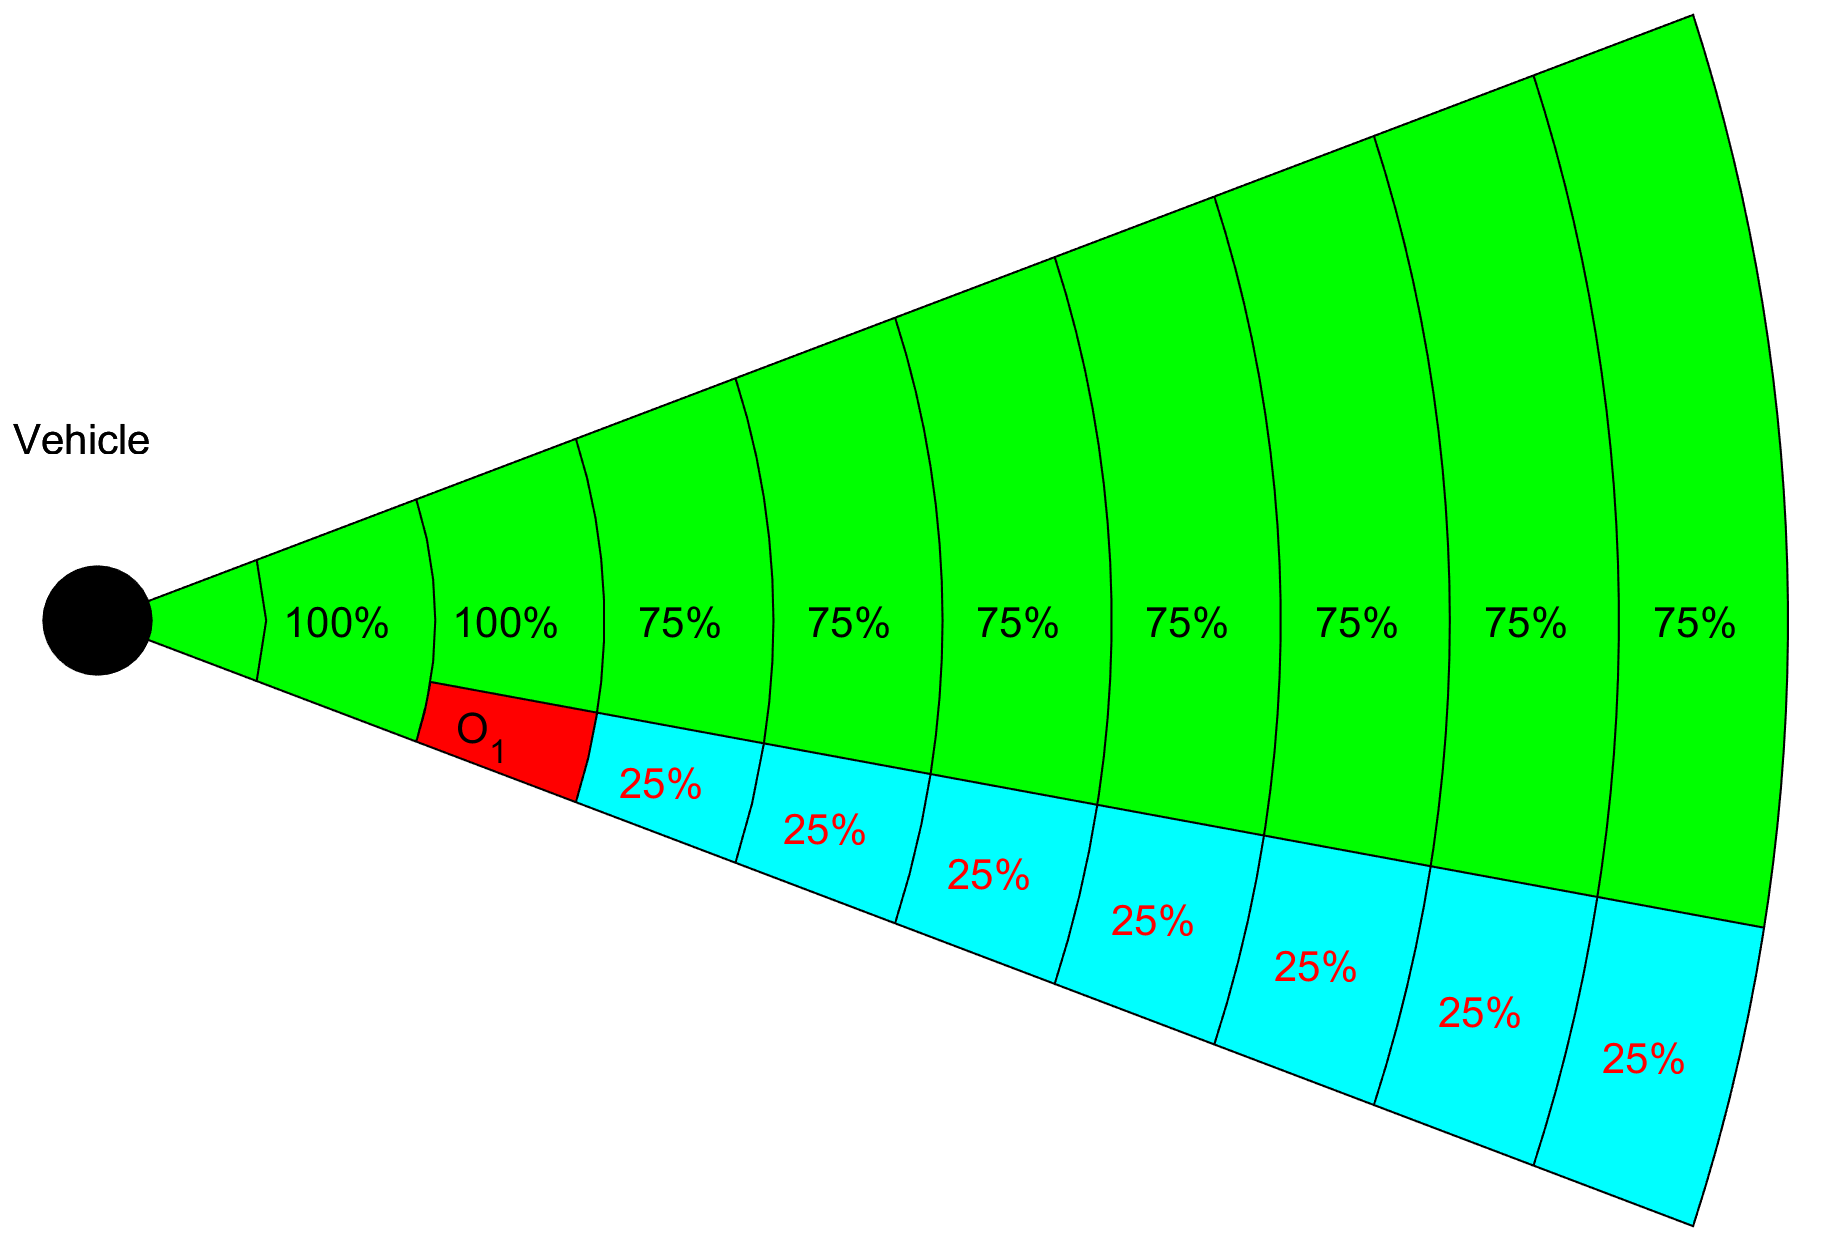
\includegraphics[width=0.9\linewidth]{\FIGDIR/TE006VisibilityFirstObstacle} 
            \caption{1\textsuperscript{st} hindrance.}
            \label{fig:fistObstacleHindrance}
        \end{subfigure}
        \begin{subfigure}{0.32\textwidth}
            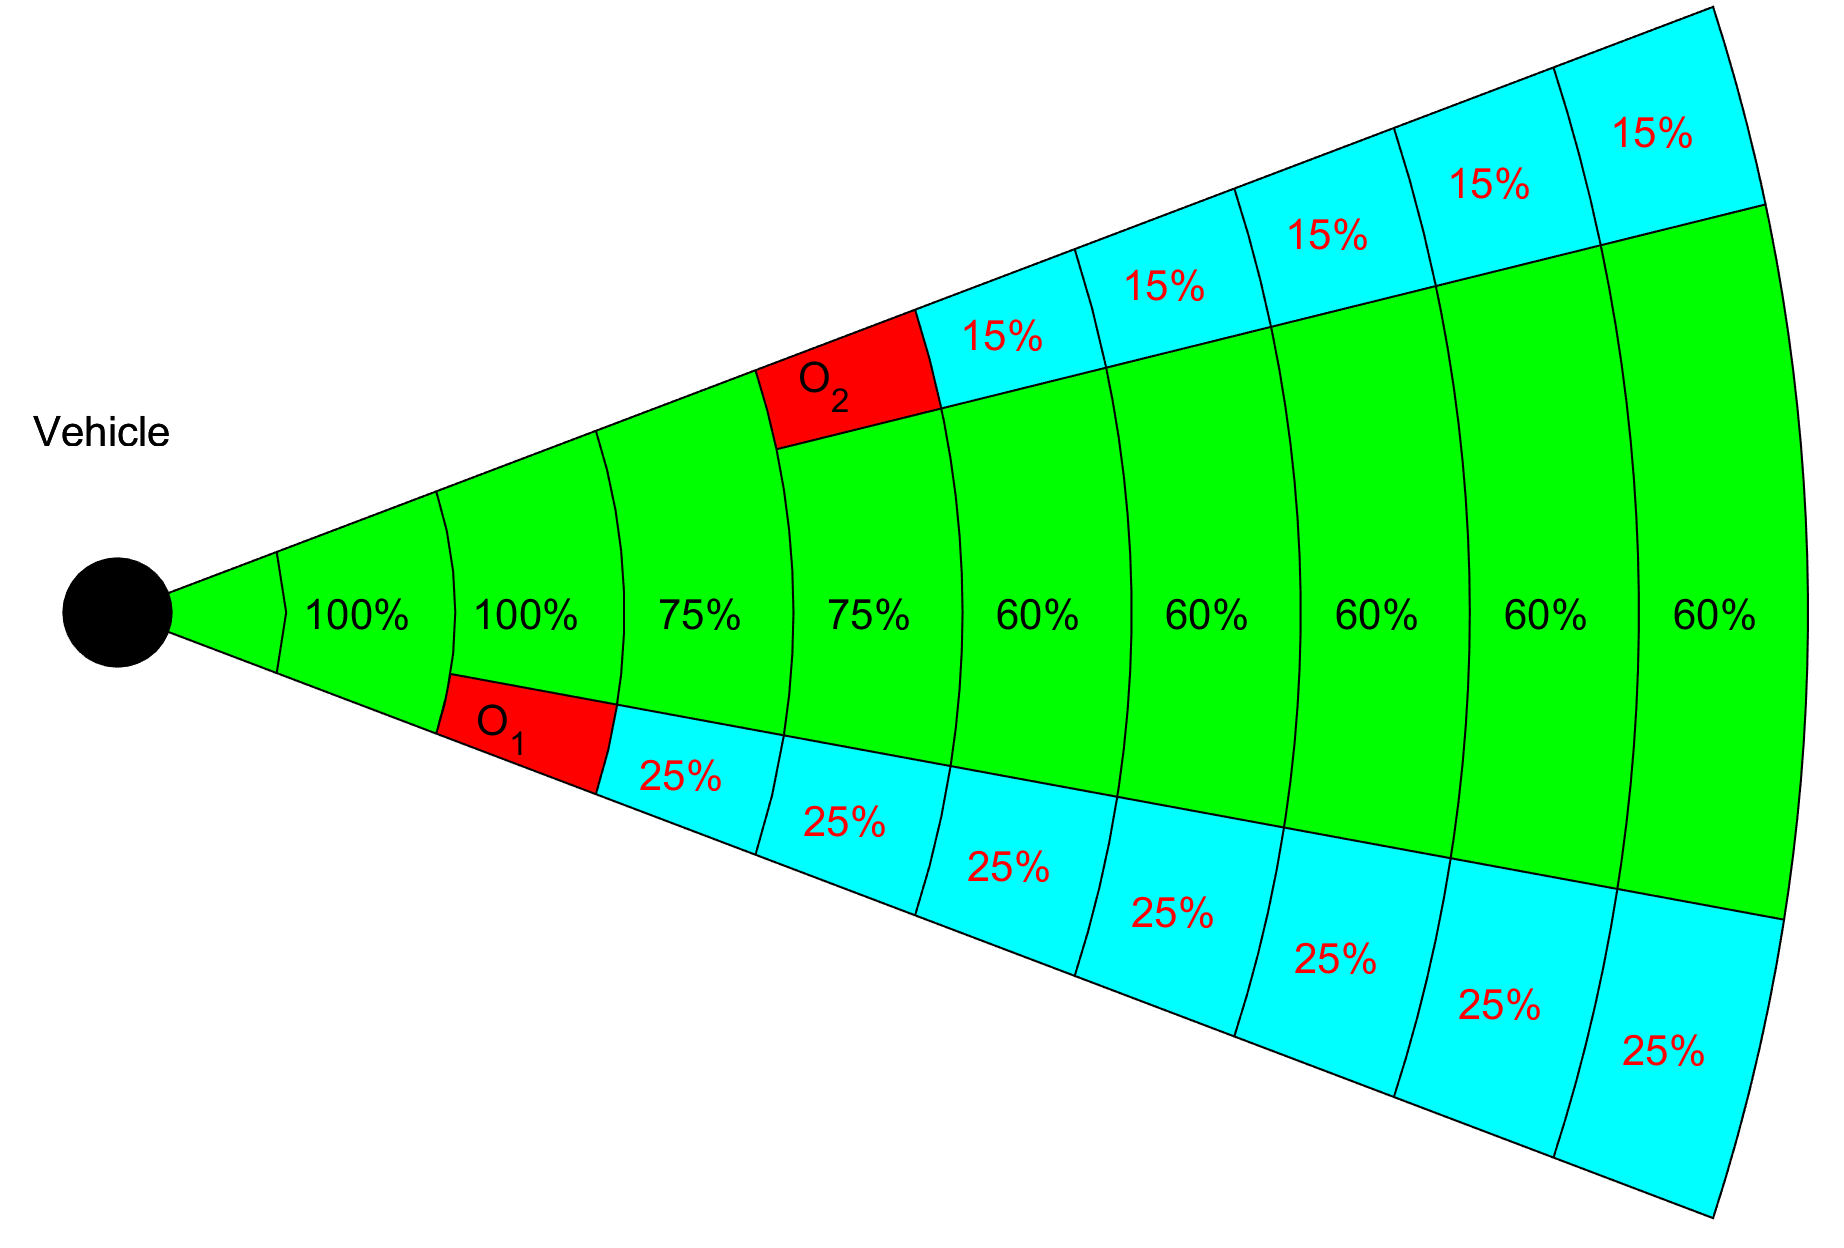
\includegraphics[width=0.9\linewidth]{\FIGDIR/TE007VisibilitySecondObstacle} 
            \caption{2\textsuperscript{nd} hindrance.}
            \label{fig:secondObstacleHindrance}
        \end{subfigure}
        \begin{subfigure}{0.32\textwidth}
            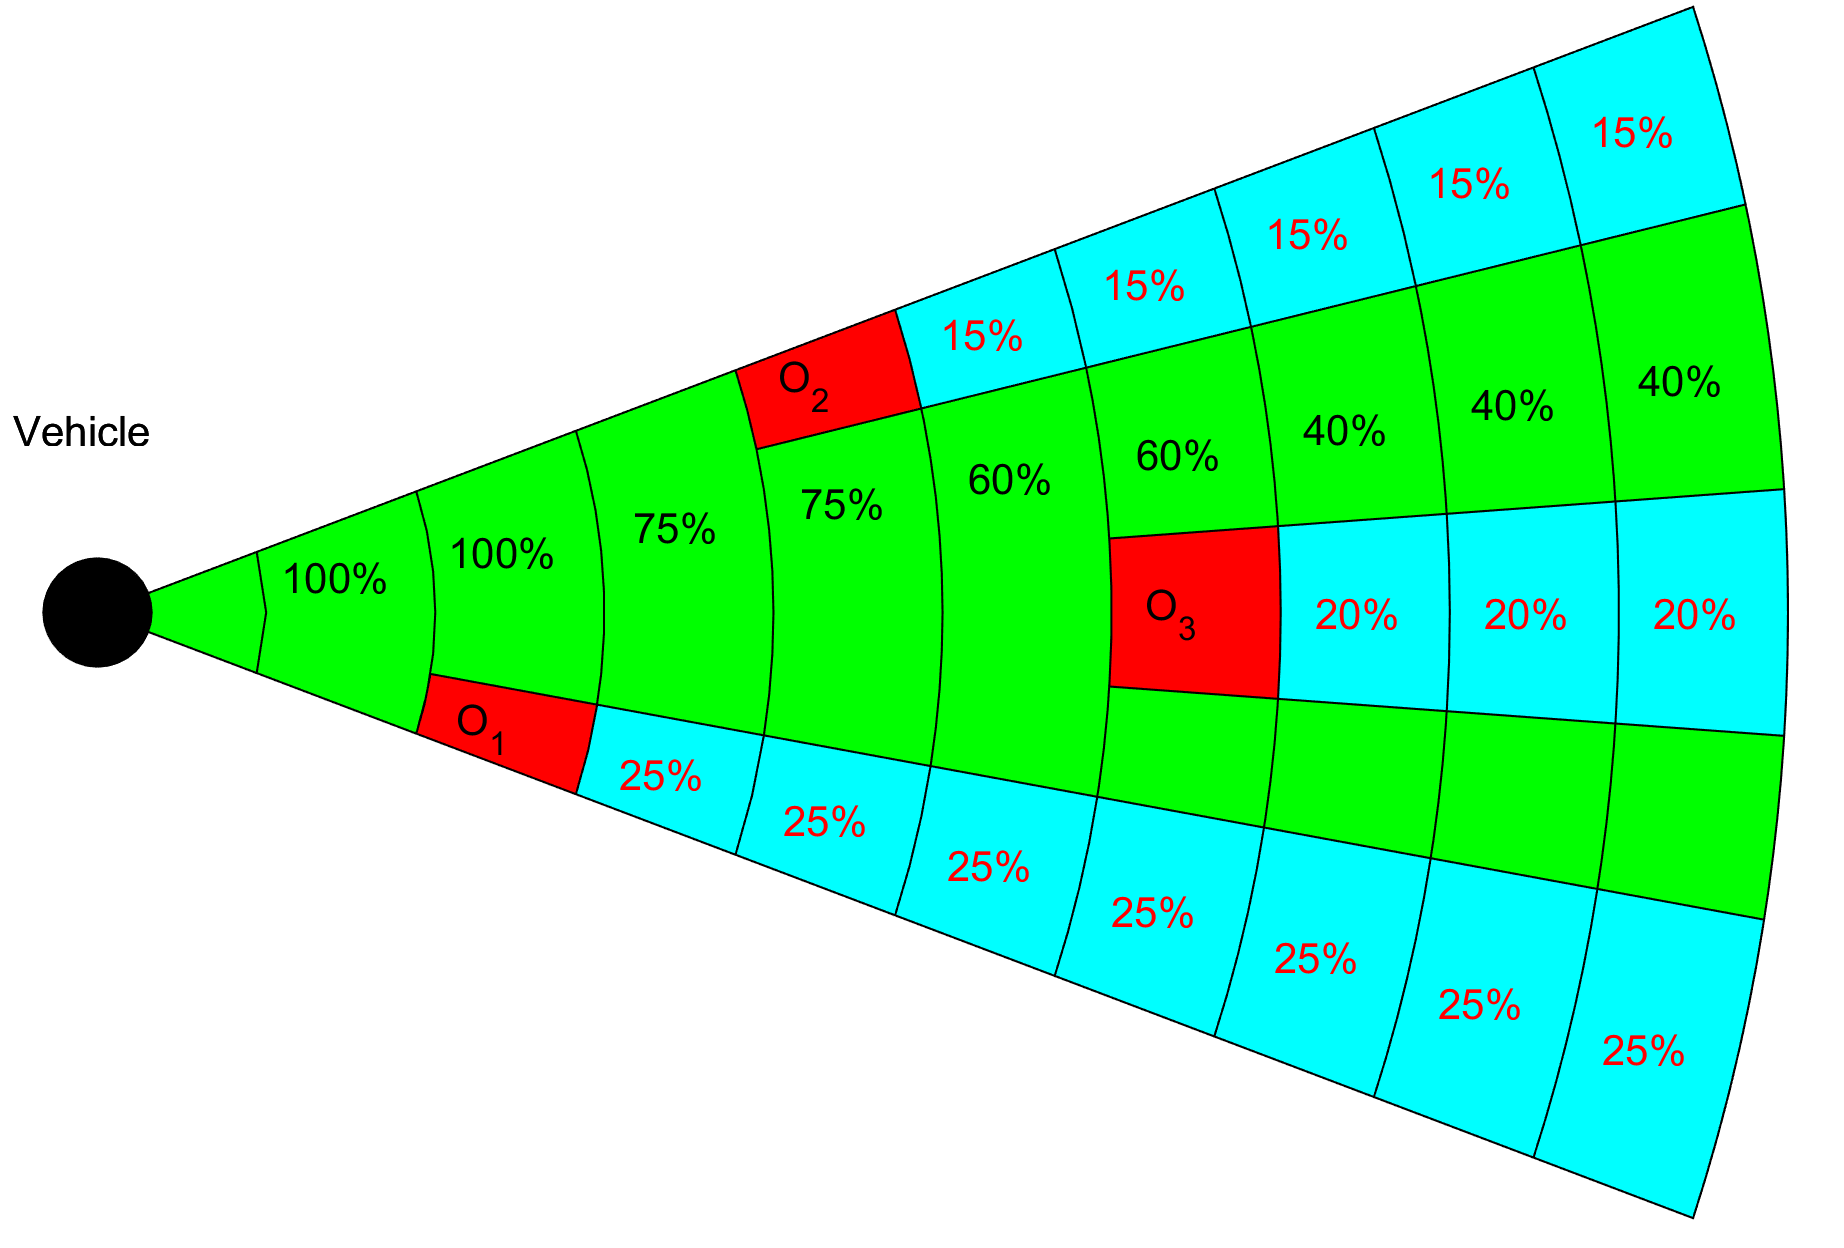
\includegraphics[width=0.9\linewidth]{\FIGDIR/TE008VisibilityThirdObstacle} 
            \caption{3\textsuperscript{rd} hindrance.}
            \label{fig:thirdObstacleHindrance}
        \end{subfigure}
        \caption{Obstacle hindrance impact on visibility in \emph{Avoidance Grid Slice}.}
        \label{fig:hindranceImpactOnVisibility}
    \end{figure}
    
    
    \begin{figure}[H]
        \begin{subfigure}{0.32\textwidth}
            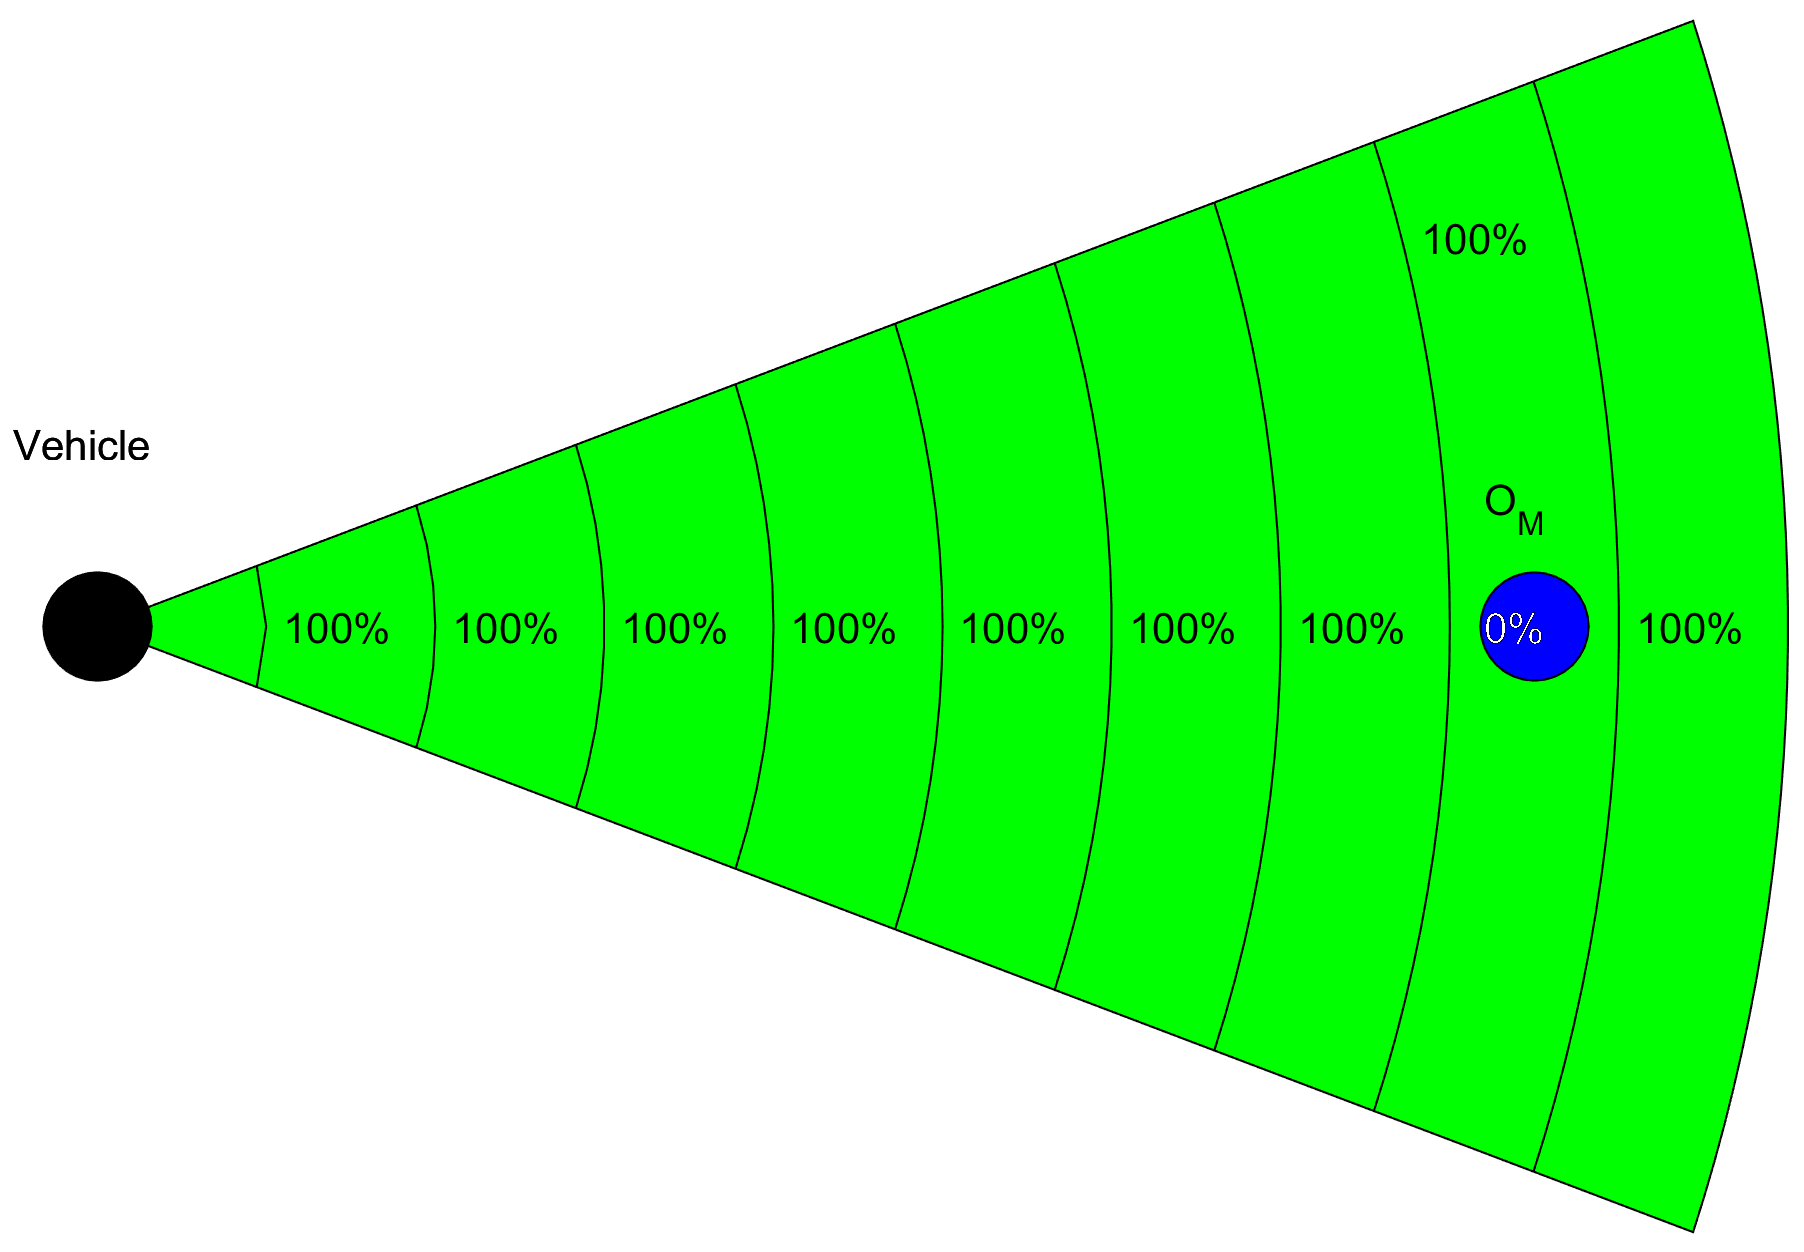
\includegraphics[width=0.9\linewidth]{\FIGDIR/TE009MapObstacleUndetected} 
            \caption{Undetected.}
            \label{fig:undetectedMapObstalce.}
        \end{subfigure}
        \begin{subfigure}{0.32\textwidth}
            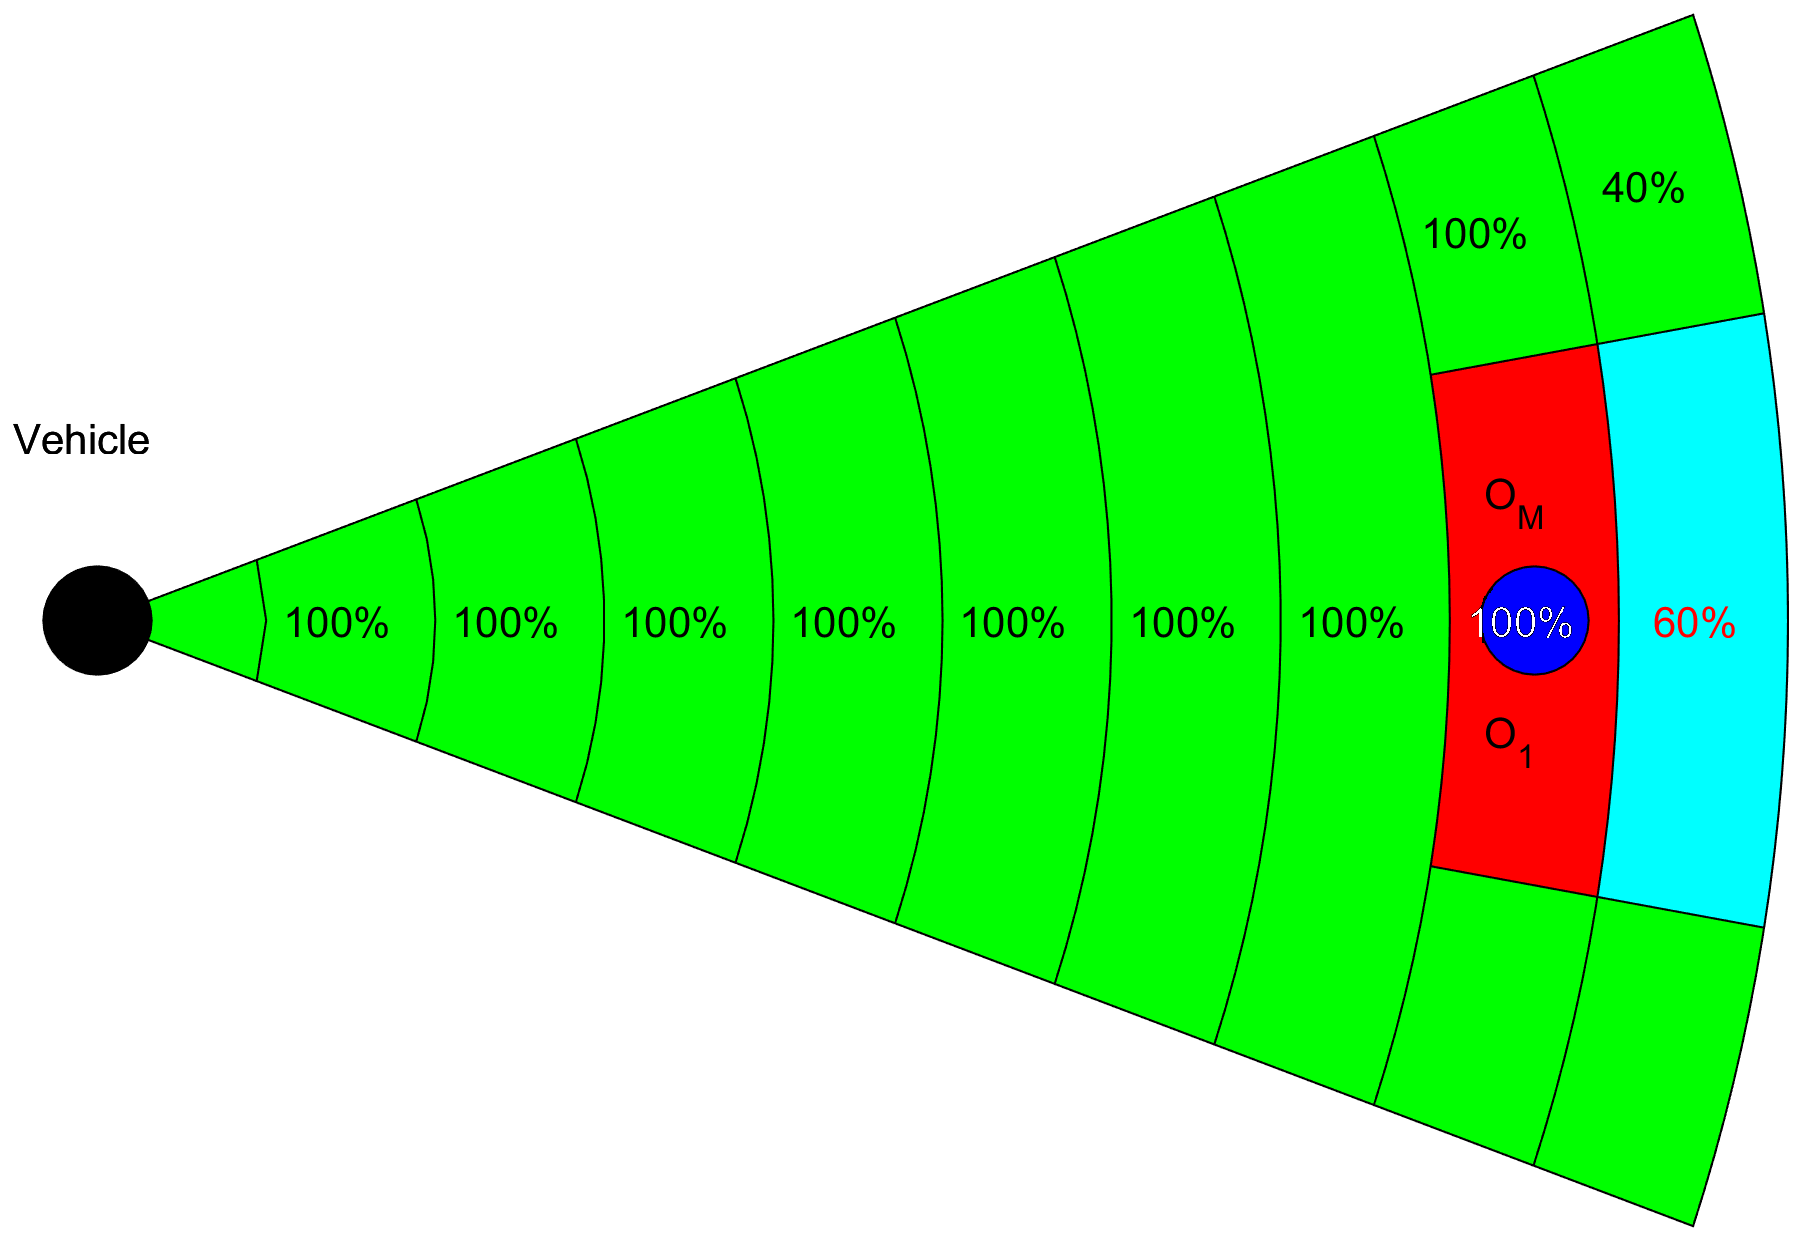
\includegraphics[width=0.9\linewidth]{\FIGDIR/TE010MapObstacleDetected} 
            \caption{Detected.}
            \label{fig:detectedMapObstacle}
        \end{subfigure}
        \begin{subfigure}{0.32\textwidth}
            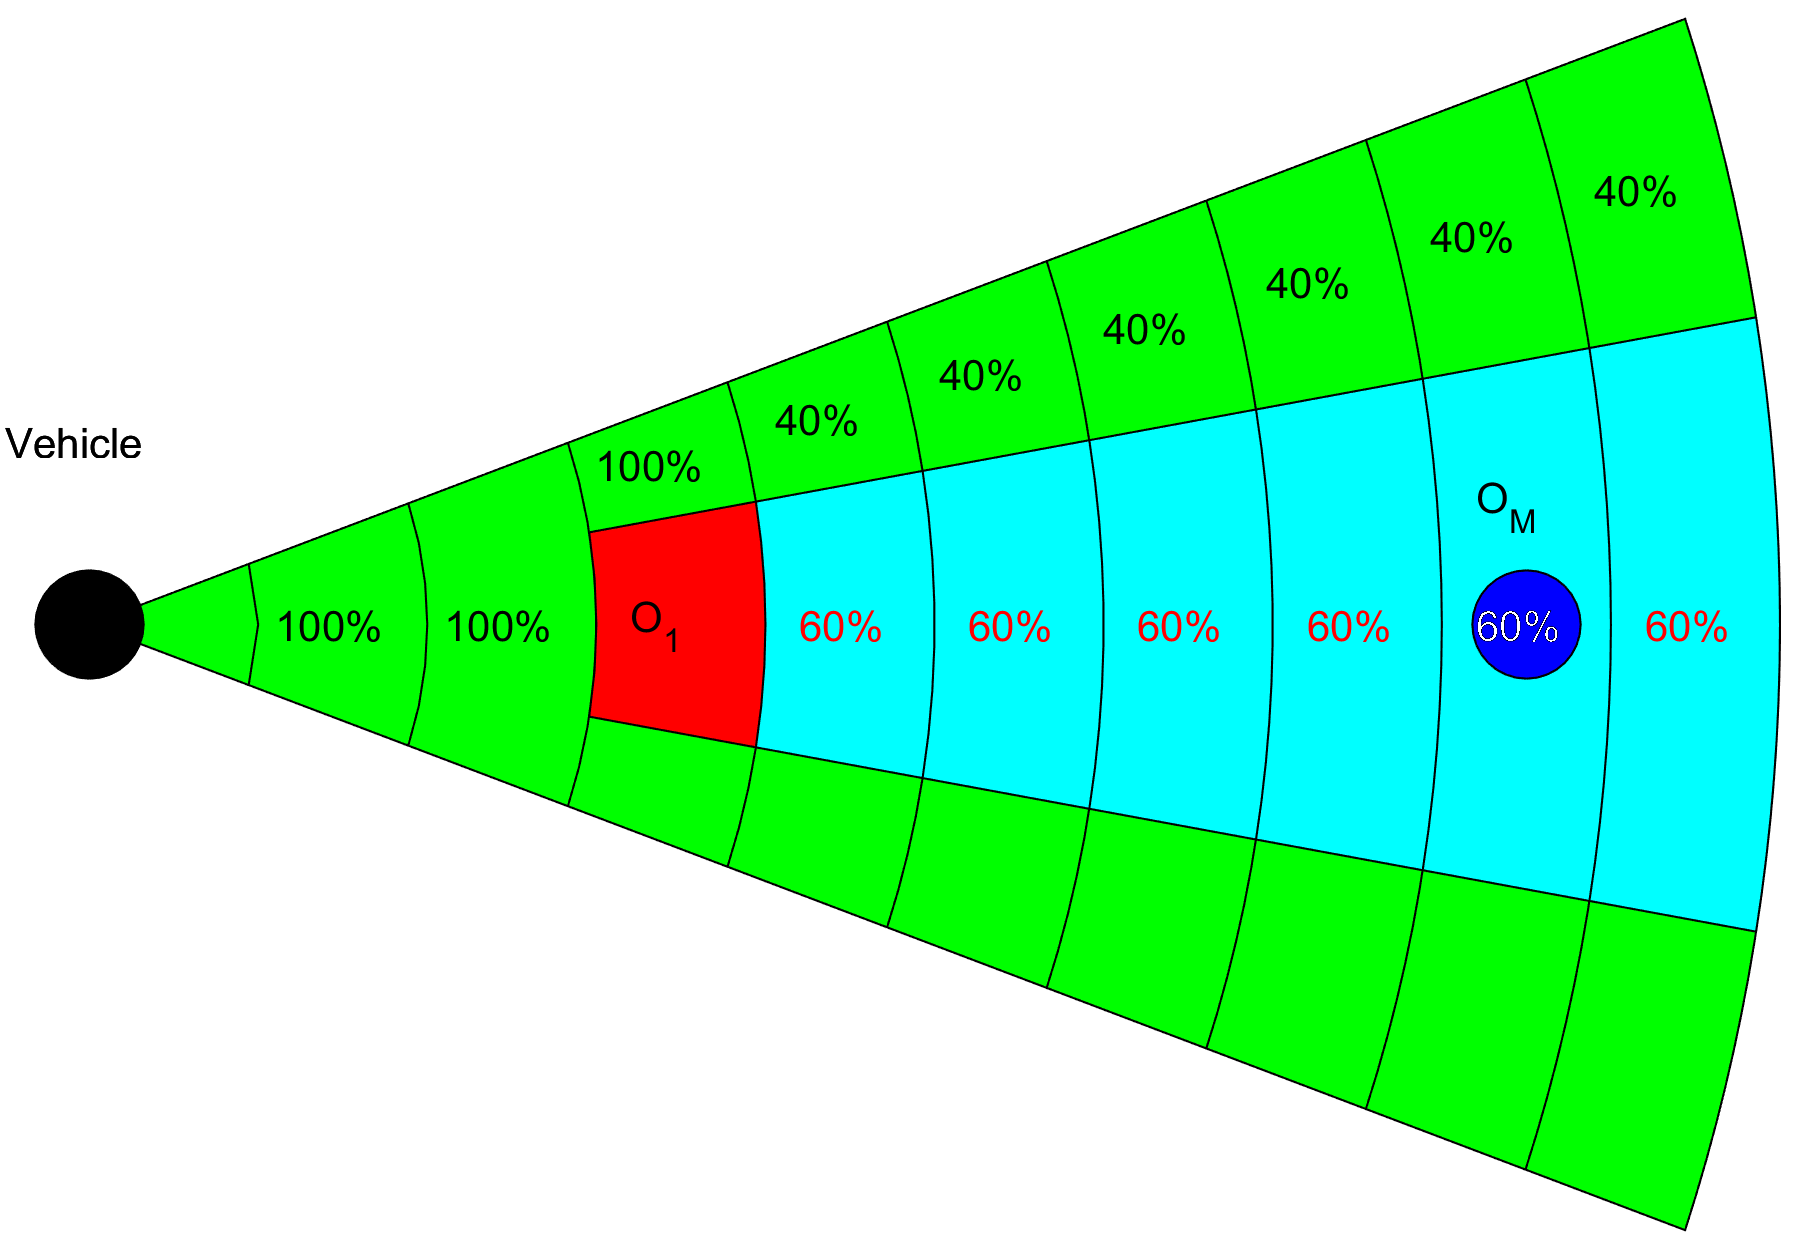
\includegraphics[width=0.9\linewidth]{\FIGDIR/TE011MapObstacleHiden}
            \caption{Hindered.}
            \label{fig:hinderedMapObstacle}
        \end{subfigure}
        \caption{Map obstacle states after \emph{Data fusion}.}
        \label{fig:mapObstacleStatesAfterDataFusion}
    \end{figure}


The \emph{Map Obstacle} were taken from my \emph{master student} \cite{cernamaria2018}
    
\begin{figure}[H]
    \centering
    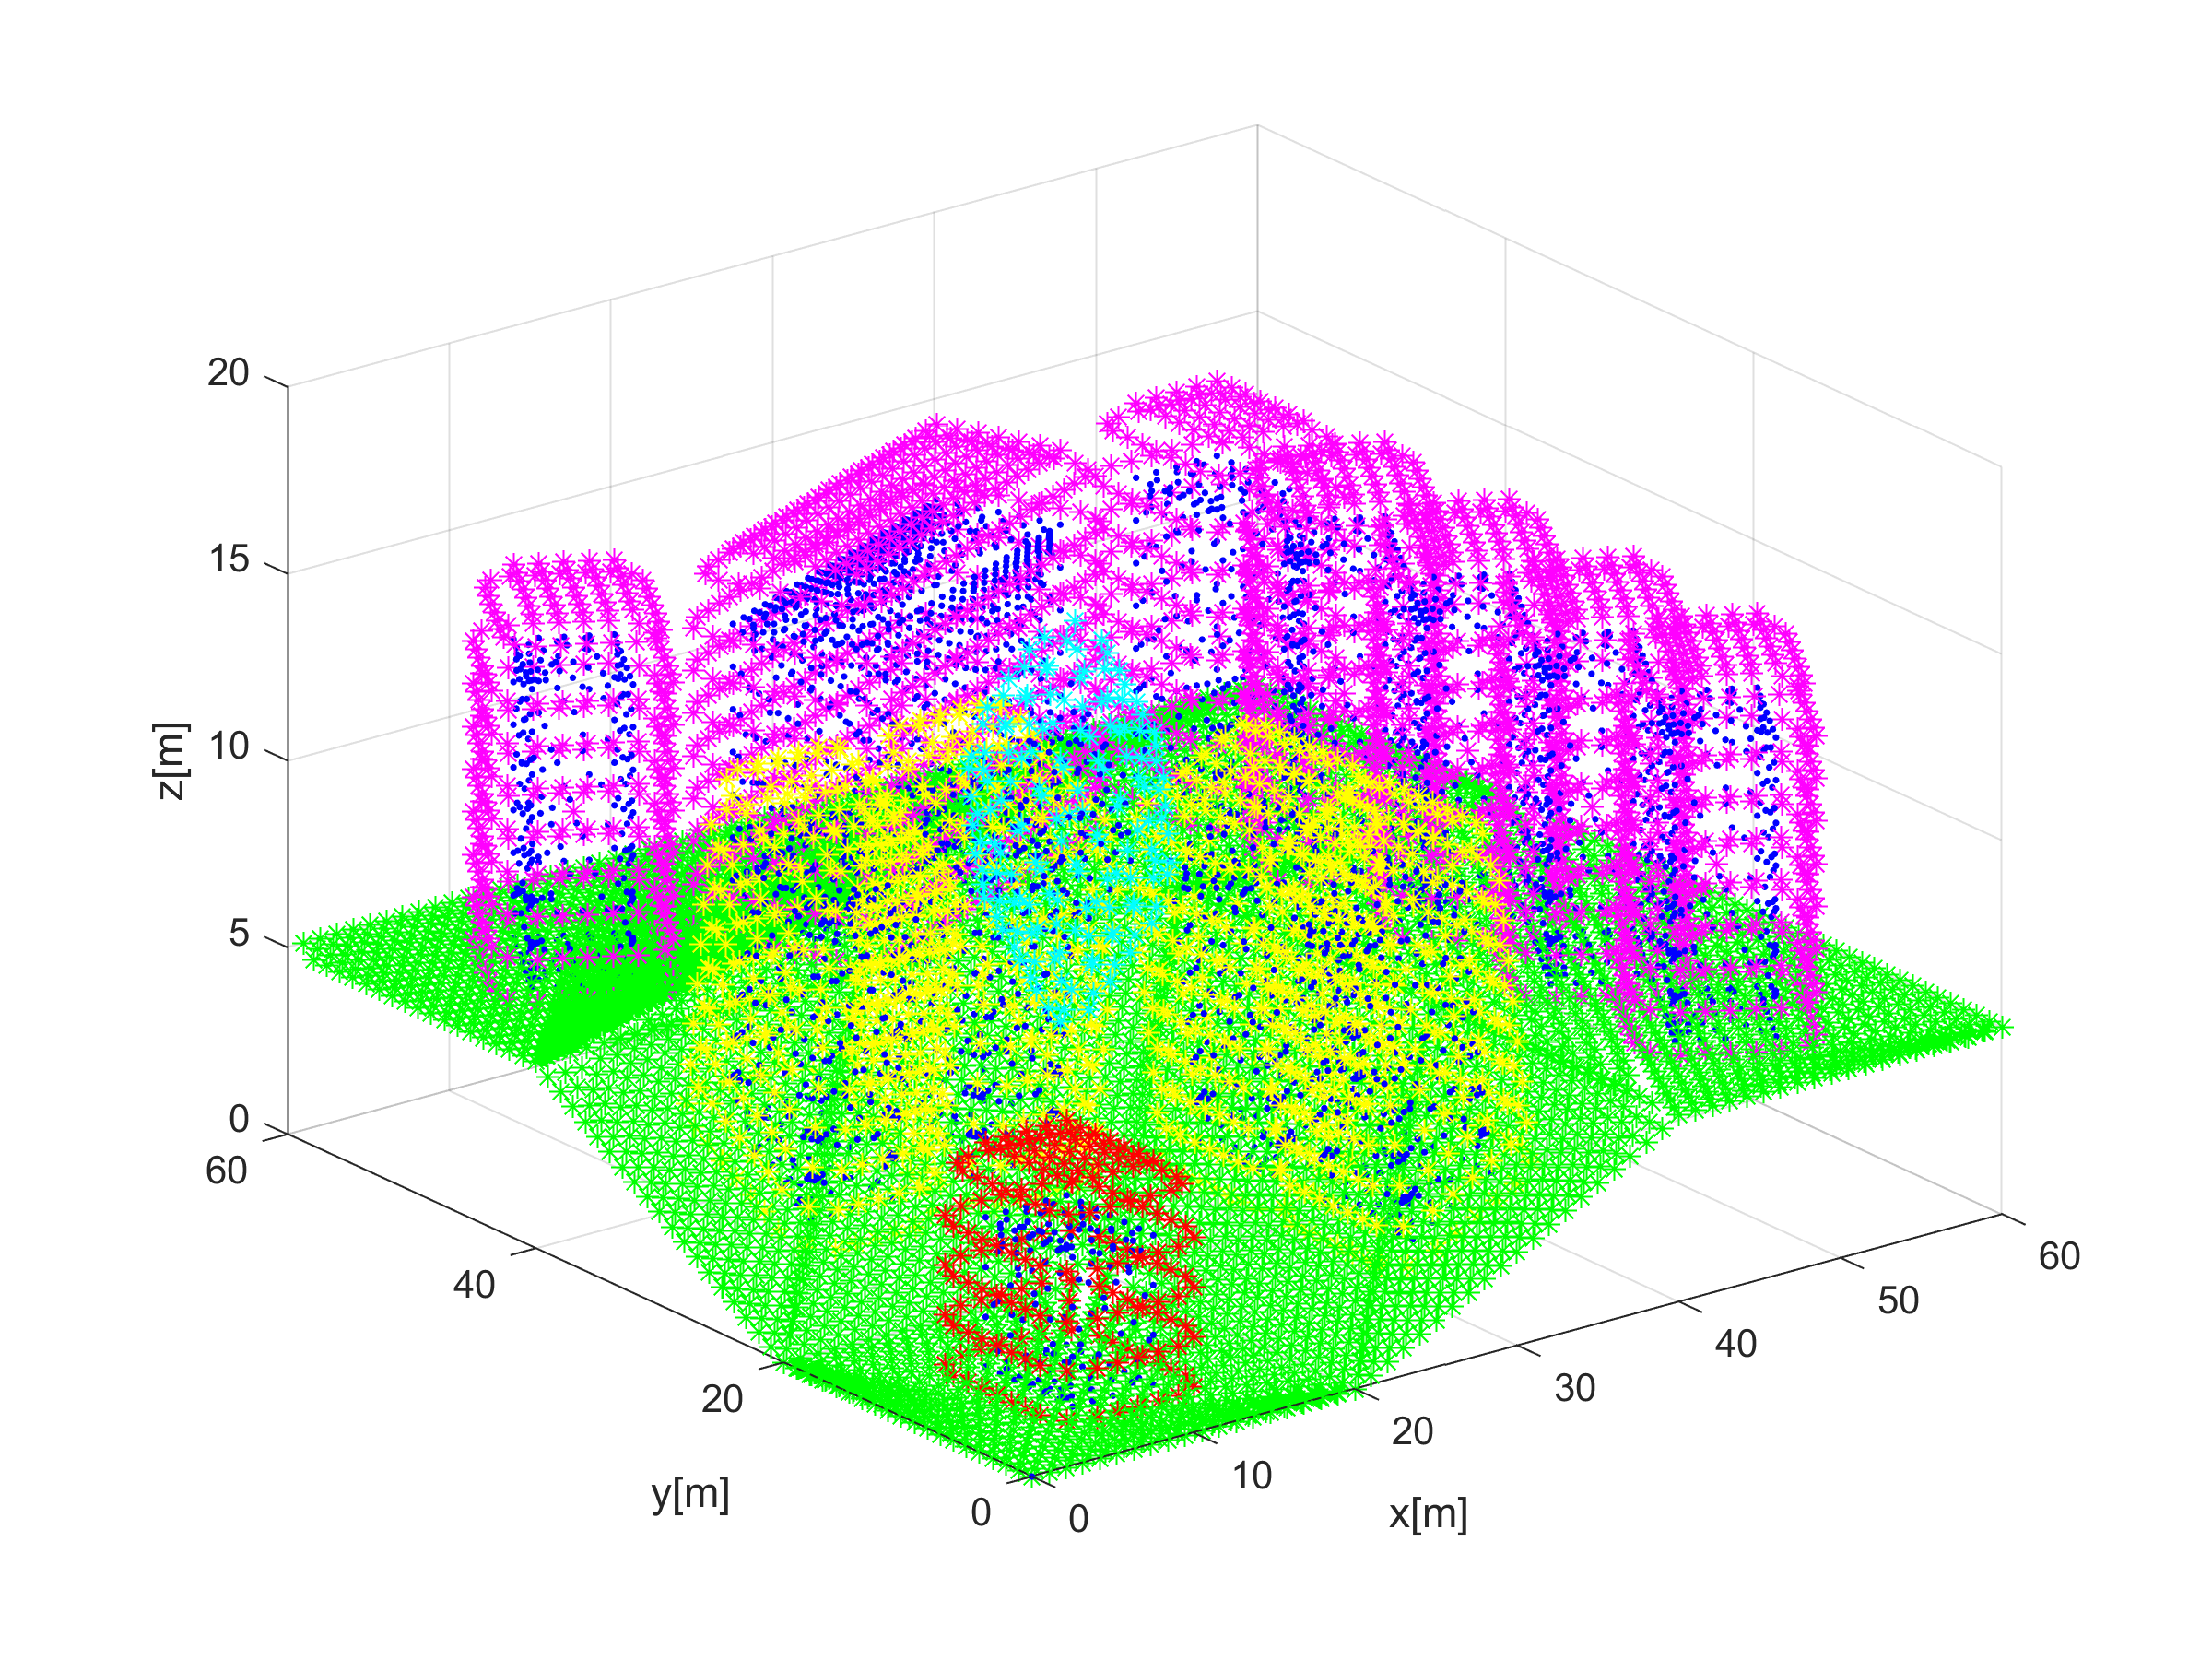
\includegraphics[width=0.7\textwidth]{\FIGDIR/TE054ExtractedMapObstaclesExample}
    \caption{Example of Extracted Map Obstacle \cite{cernamaria2018}.}
    \label{fig:exampleExtractedMapObstacles}
\end{figure} 
